\section{Simulation}
\FloatBarrier
\subsection{GEMC: Event Generation}
Events are generated using the GEMC software which uses \textit{gcard} using the command:
\begin{verbatim}
       gemc gcard/fc-ecpcsc-s2.gcard -RUNNO=12 -N=5000000 -USE_GUI=0
\end{verbatim}
The attenuation constants extracted from the data are saved in the database as CCDB constants. These constants 
(gains normalized to 100) are picked up by the \textit{gcard} with \texttt{RUNN0=12}. When executed with the above command, 5000000 events
are produced. A snapshot of the code snipped is shown in Fig.~\ref{fig:gcard}. A total of 3 million events are
generated in module 2 of the PCAL unit in order to do the simulation studies.

\begin{figure}[h]
    \centering
    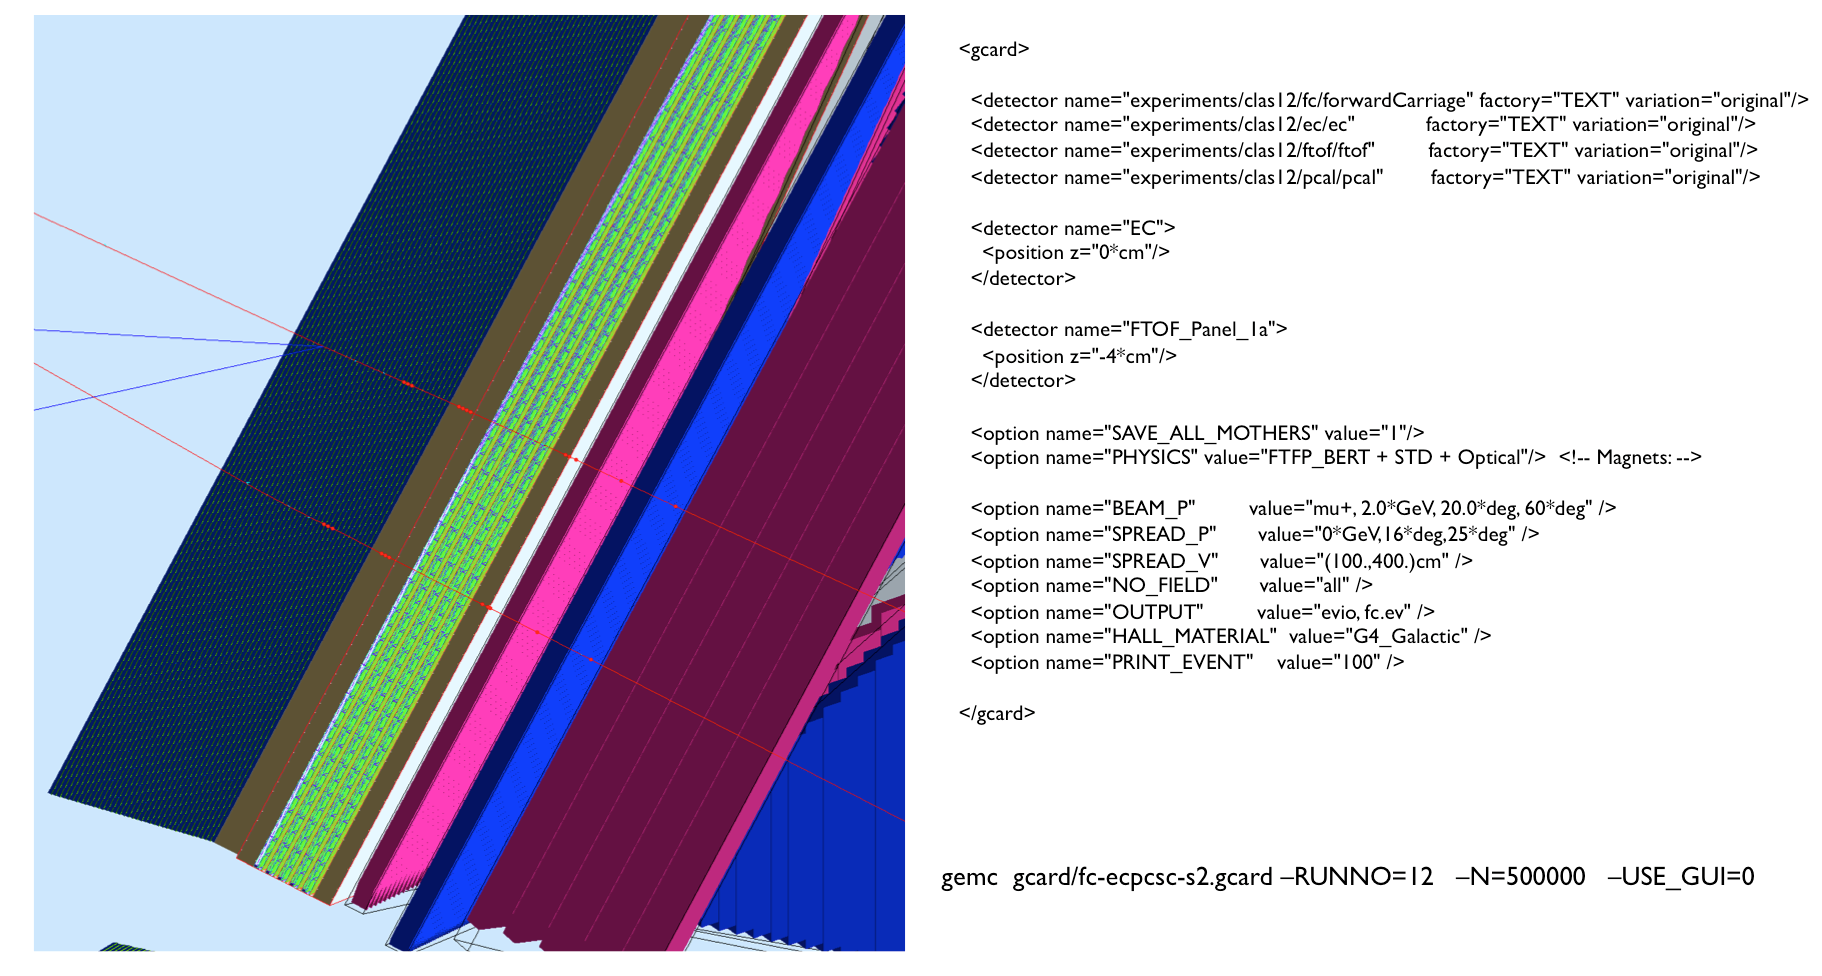
\includegraphics[width= 7in, keepaspectratio = true]{gcard}
    \caption{Snippet of the code to produce simulated events using GEMC. The graphic shows two muon tracks passing from 
    right to left.}
    \label{fig:gcard}
\end{figure}
\FloatBarrier

\FloatBarrier
\subsection{Input: Generation coefficient}
The attenuation coefficients given in Tables~\ref{tab:UattenC},~\ref{tab:VattenC} and \ref{tab:WattenC} are used as the generation
coefficients. In the attenuation equation,
\begin{equation}
y = A e^{Bx} + C
\label{eq:attn}
\end{equation}
$A$, $B$ and $C$ are the attenuation coefficients and $A+C$ is defined as the gain. The gain was normalized to an \textit{ad hoc}
factor of 100. The normalized values are fed as the generation input, which, as previously mentioned, are picked up by the
\textit{gcard}.
\FloatBarrier

\FloatBarrier
\subsection{Cuts Applied}
Different cuts wherever relevant should be applied to ensure a more accurate calibration. The ADC distributions of the 
generated events are much clean as they contain no or almost negligible background. However, to be consistent with the method
used for the calibration of the data, two cuts are made so far. These cuts are discussed below:

\subsubsection{Multiplicity Cut}
Events with exactly one U-hit, one V-hit and one W-hit are only selected. This will also help to reduce/remove events which are not
relatively perpendicular to the surface of the PCAL module. Events which do not pass this cut are removed from the analysis.

\subsubsection{Valid Pixel Cut}
\textcolor{red}{Explain about the HitMatrix first.} Another condition required for the events to be selected is that they are
within the physical shape made by the overlap. The true physical shape, pixel or an overlap shape, is given in the DataBase in the 
form of a matrix known as the \textit{hit-matrix}. Events that do not fall within these shapes are removed from the analysis. This cut
is another way of using the Dalitz cut.
\FloatBarrier

\FloatBarrier
\subsection{ADC and Exponential fits}
The events which pass the cuts are binned according to which strip is being calibrated. For example, to calibrate U-strips, bins of W
cross-strips are used. The ADC signals in those bins are plotted and centroids are extracted. The centroids are then plotted as a
function of distance and are fit using exponential function $y$ given in Eq.~\ref{eq:attn} and the parameters are the required
calibration constants. Figures \ref{fig:expfit1} and \ref{fig:expfit2} show the fits of ten U-strips (U51- U60). The curve in red
is the drawn using the generated coefficients fed in the GEMC.
\begin{figure}[h]
    \centering
    \begin{subfigure}[h]{0.44\textwidth}
        \centering
        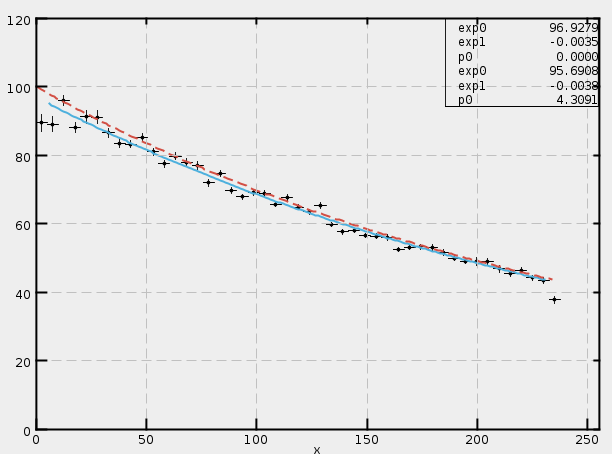
\includegraphics[width=\textwidth, keepaspectratio = true]{expfit_U51}
        \caption{expfitU51}
        \label{fig:expfit_U51}
    \end{subfigure}
    ~
    \begin{subfigure}[h]{0.44\textwidth}
        \centering
        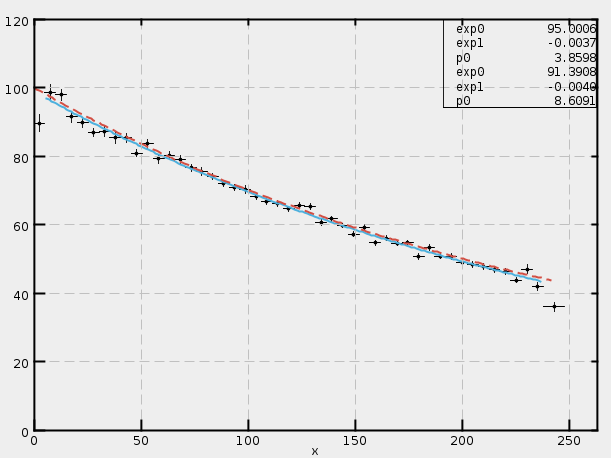
\includegraphics[width=\textwidth, keepaspectratio = true]{expfit_U52}
        \caption{expfitU52}
        \label{fig:expfit_U52}
    \end{subfigure}
    
    \begin{subfigure}[h]{0.44\textwidth}
        \centering
        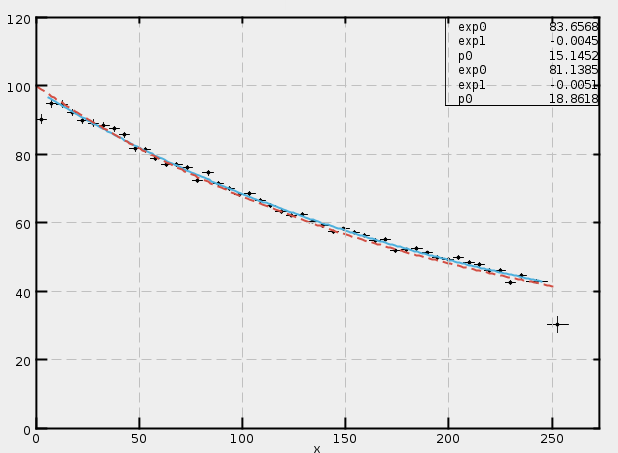
\includegraphics[width=\textwidth, keepaspectratio = true]{expfit_U53}
        \caption{expfitU53}
        \label{fig:expfit_U53}
    \end{subfigure}
    ~
    \begin{subfigure}[h]{0.44\textwidth}
        \centering
        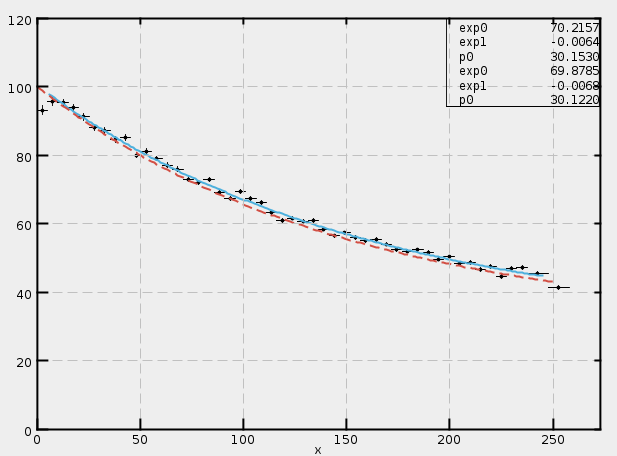
\includegraphics[width=\textwidth, keepaspectratio = true]{expfit_U54}
        \caption{expfitU54}
        \label{fig:expfit_U54}
    \end{subfigure}
    \caption{Exponential fits for strips U51-U54. The first set of three coeffcients are from the fit and the next set of three are
     the coefficients used in the event generation.}
    \label{fig:expfit1}
\end{figure}

\begin{figure}[h]
    \centering
    \begin{subfigure}[h]{0.44\textwidth}
        \centering
        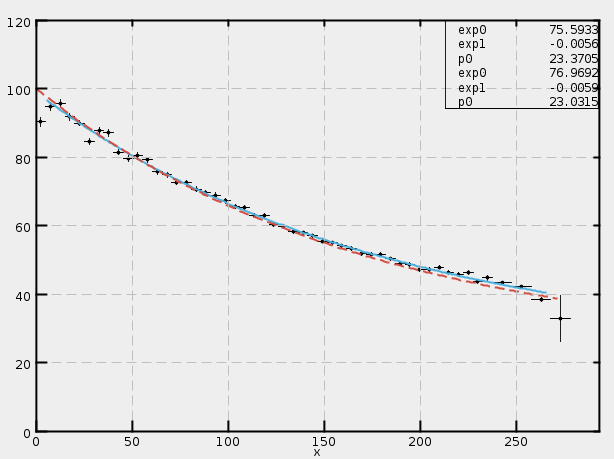
\includegraphics[width=\textwidth, keepaspectratio = true]{expfit_U55}
        \caption{expfitU55}
        \label{fig:expfit_U55}
    \end{subfigure}
    ~
    \begin{subfigure}[h]{0.44\textwidth}
        \centering
        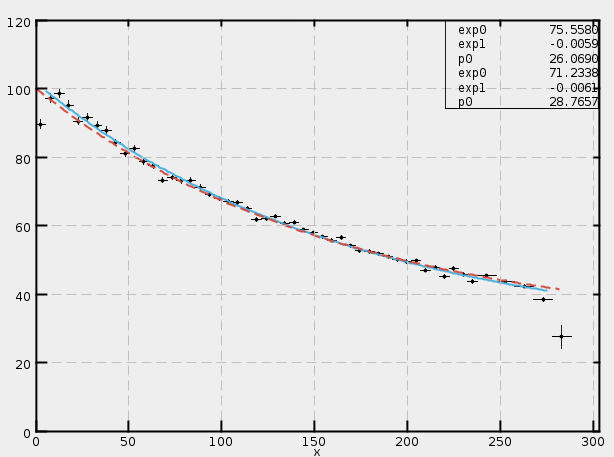
\includegraphics[width=\textwidth, keepaspectratio = true]{expfit_U56}
        \caption{expfitU56}
        \label{fig:expfit_U56}
    \end{subfigure}
    
    \begin{subfigure}[h]{0.44\textwidth}
        \centering
        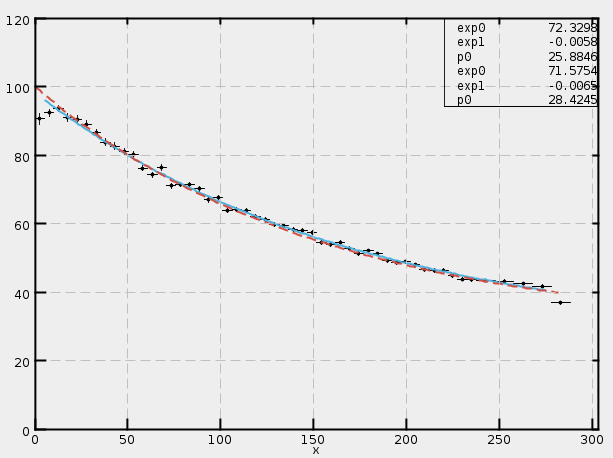
\includegraphics[width=\textwidth, keepaspectratio = true]{expfit_U57}
        \caption{expfitU57}
        \label{fig:expfit_U57}
    \end{subfigure}
    ~
    \begin{subfigure}[h]{0.44\textwidth}
        \centering
        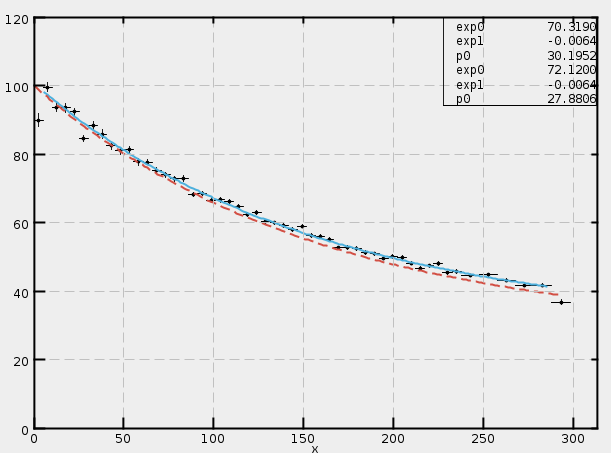
\includegraphics[width=\textwidth, keepaspectratio = true]{expfit_U58}
        \caption{expfitU58}
        \label{fig:expfit_U58}
    \end{subfigure}
    
    \begin{subfigure}[h]{0.44\textwidth}
        \centering
        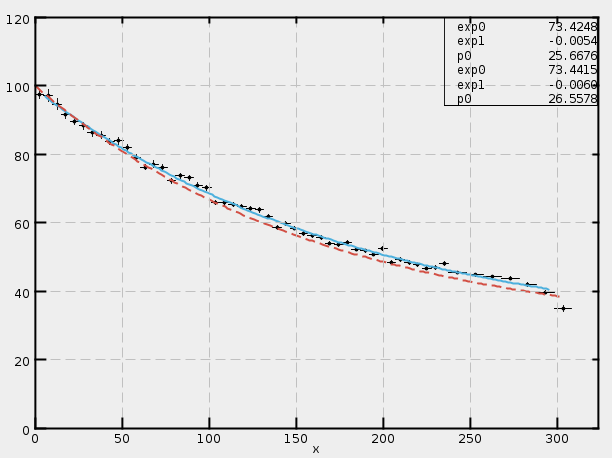
\includegraphics[width=\textwidth, keepaspectratio = true]{expfit_U59}
        \caption{expfitU59}
        \label{fig:expfit_U59}
    \end{subfigure}
    ~
    \begin{subfigure}[h]{0.44\textwidth}
        \centering
        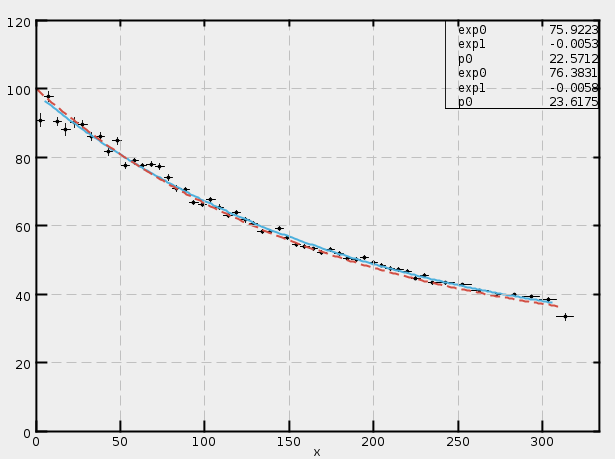
\includegraphics[width=\textwidth, keepaspectratio = true]{expfit_U60}
        \caption{expfitU60}
        \label{fig:expfit_U60}
    \end{subfigure}
    \caption{Exponential fits for strips U55-U60. The first set of three coeffcients are from the fit and the next set of three are
     the coefficients used in the event generation.}
    \label{fig:expfit2}
\end{figure}
\FloatBarrier

\FloatBarrier
\subsection{Attenuation Coeffiecients}
\textcolor{red}{Tables showing the attenuation coefficients.}
\begin{table}[h]
        \centering{}
        \scalebox{0.75}{
        \begin{tabular}{|c|c|c|c|}
            \hline
            U-Strip &  Parameter $a$  &Parameter $b$  & Parameter $c$ \\ \hline
1   &   650   &   0   &   0  \\  \hline  
2   &   650   &   0   &   0  \\  \hline  
3   &   650   &   -0.009   &   0  \\  \hline  
4   &   650   &   -0.009   &   0  \\  \hline  
5   &   616.113   &   -0.00639717   &   33.8858  \\  \hline  
6   &   649.996   &   -0.00717551   &   0.0046356  \\  \hline  
7   &   649.968   &   -0.00318808   &   0.0319326  \\  \hline  
8   &   649.972   &   -0.00232476   &   0.0273016  \\  \hline  
9   &   649.146   &   -0.00112904   &   0.854413  \\  \hline  
10   &   649.999   &   -0.00281005   &   0.000286188  \\  \hline  
11   &   649.993   &   -0.00286292   &   0.00718601  \\  \hline  
12   &   650   &   -0.0041656   &   0.000445736  \\  \hline  
13   &   650   &   -0.003283   &   0.000103724  \\  \hline  
14   &   649.997   &   -0.00376077   &   5.37227e-06  \\  \hline  
15   &   650.001   &   -0.00339912   &   6.96689e-06  \\  \hline  
16   &   649.997   &   -0.00305411   &   8.14649e-06  \\  \hline  
17   &   649.999   &   -0.00345134   &   9.95183e-09  \\  \hline  
18   &   649.998   &   -0.00310718   &   4.19396e-07  \\  \hline  
19   &   650   &   -0.00311517   &   5.01049e-06  \\  \hline  
20   &   650   &   -0.00281725   &   6.09084e-06  \\  \hline  
21   &   650   &   -0.00315783   &   3.38135e-05  \\  \hline  
22   &   650   &   -0.00328681   &   2.55834e-08  \\  \hline  
23   &   650   &   -0.00316776   &   2.15877e-05  \\  \hline  
24   &   649.999   &   -0.00317021   &   4.66803e-05  \\  \hline  
25   &   650   &   -0.00327065   &   5.9556e-06  \\  \hline  
26   &   650.001   &   -0.00309179   &   1.40689e-08  \\  \hline  
27   &   551.087   &   -0.00385902   &   98.9141  \\  \hline  
28   &   649.997   &   -0.00307714   &   7.49416e-05  \\  \hline  
29   &   419.522   &   -0.00552754   &   230.477  \\  \hline  
30   &   650   &   -0.00316014   &   0.000130702  \\  \hline  
31   &   650.001   &   -0.00312815   &   2.25921e-06  \\  \hline  
32   &   585.658   &   -0.00373922   &   64.3455  \\  \hline  
33   &   581.001   &   -0.00374214   &   68.997  \\  \hline  
34   &   650.002   &   -0.00328878   &   0.000131253  \\  \hline  
35   &   650   &   -0.00332314   &   1.43305e-05  \\  \hline  
36   &   649.998   &   -0.00340294   &   1.07435e-07  \\  \hline  
37   &   556.399   &   -0.00428136   &   93.5991  \\  \hline  
38   &   483.854   &   -0.00534903   &   166.146  \\  \hline  
39   &   482.458   &   -0.00431684   &   167.541  \\  \hline  
40   &   392.765   &   -0.00669036   &   257.235  \\  \hline  
41   &   499.22   &   -0.00443664   &   150.78  \\  \hline  
42   &   513.839   &   -0.00445738   &   136.164  \\  \hline  
43   &   581.507   &   -0.00388427   &   68.4914  \\  \hline  
44   &   391.463   &   -0.00757633   &   258.536  \\  \hline  
45   &   434.393   &   -0.00632194   &   215.608  \\  \hline  
46   &   463.813   &   -0.00513914   &   186.187  \\  \hline  
47   &   413.809   &   -0.00605594   &   236.189  \\  \hline  
48   &   442.234   &   -0.00592955   &   207.766  \\  \hline  
49   &   509.976   &   -0.00449146   &   140.024  \\  \hline  
50   &   443.895   &   -0.00614484   &   206.105  \\  \hline  
51   &   425.765   &   -0.00641114   &   224.233  \\  \hline  
52   &   504.812   &   -0.00511618   &   145.188  \\  \hline  
53   &   454.838   &   -0.0061679   &   195.162  \\  \hline  
54   &   406.411   &   -0.00766326   &   243.589  \\  \hline  
55   &   415.976   &   -0.00690821   &   234.026  \\  \hline  
56   &   421.326   &   -0.00710769   &   228.675  \\  \hline  
57   &   435.635   &   -0.00660386   &   214.362  \\  \hline  
58   &   411.518   &   -0.00663318   &   238.483  \\  \hline  
59   &   438.882   &   -0.00625669   &   211.118  \\  \hline  
60   &   423.763   &   -0.00618908   &   226.238  \\  \hline  
61   &   444.671   &   -0.0063621   &   205.328  \\  \hline  
62   &   438.481   &   -0.00674885   &   211.519  \\  \hline  
63   &   437.138   &   -0.00564978   &   212.862  \\  \hline  
64   &   482.525   &   -0.00495599   &   167.473  \\  \hline  
65   &   473.388   &   -0.00516614   &   176.613  \\  \hline  
66   &   465.633   &   -0.00500512   &   184.367  \\  \hline  
67   &   455.941   &   -0.00479029   &   194.059  \\  \hline  
68   &   410.201   &   -0.00506009   &   239.798  \\  \hline  
        \end{tabular}
        }
        \caption{Calibration Constants for the U layer.}
        \label{tab:UattenCSimulation}
\end{table}


\begin{table}[h]
        \centering
        \scalebox{0.75}{
        \begin{tabular}{|c|c|c|c|}
            \hline
            V-Strip &  Parameter $a$  &Parameter $b$  & Parameter $c$ \\ \hline
1   &   650.002   &   0   &   0  \\  \hline  
2   &   649.999   &   0   &   0  \\  \hline  
3   &   650.001   &   -0.009   &   0  \\  \hline  
4   &   650.001   &   -0.009   &   8.41036e-07  \\  \hline  
5   &   650   &   -0.00794645   &   5.04738e-06  \\  \hline  
6   &   649.225   &   -0.00402729   &   0.773706  \\  \hline  
7   &   341.165   &   -0.009   &   308.835  \\  \hline  
8   &   649.999   &   -0.0043402   &   0.000921065  \\  \hline  
9   &   650   &   -0.00346629   &   0.00030414  \\  \hline  
10   &   409.661   &   -0.0073313   &   240.338  \\  \hline  
11   &   650   &   -0.0036951   &   0.000157707  \\  \hline  
12   &   543.255   &   -0.00487653   &   106.745  \\  \hline  
13   &   385.429   &   -0.00755387   &   264.571  \\  \hline  
14   &   462.536   &   -0.00523798   &   187.463  \\  \hline  
15   &   490.318   &   -0.00478212   &   159.682  \\  \hline  
16   &   409.407   &   -0.00682511   &   240.592  \\  \hline  
17   &   644.496   &   -0.00311038   &   5.50402  \\  \hline  
18   &   649.997   &   -0.00345834   &   1.60129e-06  \\  \hline  
19   &   650   &   -0.00314254   &   4.40293e-06  \\  \hline  
20   &   476.84   &   -0.00525174   &   173.161  \\  \hline  
21   &   504.696   &   -0.00482932   &   145.304  \\  \hline  
22   &   501.641   &   -0.00447931   &   148.359  \\  \hline  
23   &   427.011   &   -0.00618067   &   222.989  \\  \hline  
24   &   532.597   &   -0.00429752   &   117.404  \\  \hline  
25   &   452.731   &   -0.00555935   &   197.267  \\  \hline  
26   &   514.63   &   -0.00444436   &   135.371  \\  \hline  
27   &   562.158   &   -0.00411837   &   87.8438  \\  \hline  
28   &   552.525   &   -0.00397784   &   97.4754  \\  \hline  
29   &   505.009   &   -0.00490977   &   144.992  \\  \hline  
30   &   545.684   &   -0.00417772   &   104.316  \\  \hline  
31   &   520.37   &   -0.00441109   &   129.628  \\  \hline  
32   &   545.125   &   -0.00412529   &   104.875  \\  \hline  
33   &   454.001   &   -0.00531295   &   195.999  \\  \hline  
34   &   430.052   &   -0.00591867   &   219.949  \\  \hline  
35   &   472.603   &   -0.00523221   &   177.394  \\  \hline  
36   &   479.173   &   -0.0044464   &   170.826  \\  \hline  
37   &   472.073   &   -0.00500161   &   177.926  \\  \hline  
38   &   521.65   &   -0.00433543   &   128.35  \\  \hline  
39   &   523.67   &   -0.00413843   &   126.33  \\  \hline  
40   &   475.448   &   -0.00450584   &   174.551  \\  \hline  
41   &   463.401   &   -0.0051012   &   186.6  \\  \hline  
42   &   486.03   &   -0.0046867   &   163.97  \\  \hline  
43   &   474.905   &   -0.00454652   &   175.094  \\  \hline  
44   &   512.336   &   -0.00460079   &   137.664  \\  \hline  
45   &   518.211   &   -0.00460405   &   131.79  \\  \hline  
46   &   503.032   &   -0.00487218   &   146.968  \\  \hline  
47   &   501.666   &   -0.00500745   &   148.335  \\  \hline  
48   &   488.139   &   -0.00450074   &   161.861  \\  \hline  
49   &   479.791   &   -0.00489837   &   170.209  \\  \hline  
50   &   487.47   &   -0.00479649   &   162.531  \\  \hline  
51   &   516.592   &   -0.0043148   &   133.409  \\  \hline  
52   &   504.835   &   -0.0045441   &   145.166  \\  \hline  
53   &   516.386   &   -0.00442848   &   133.615  \\  \hline  
54   &   493.162   &   -0.0051403   &   156.838  \\  \hline  
55   &   475.544   &   -0.00530062   &   174.455  \\  \hline  
56   &   483.85   &   -0.00428974   &   166.15  \\  \hline  
57   &   493.428   &   -0.00469419   &   156.572  \\  \hline  
58   &   485.197   &   -0.00470872   &   164.802  \\  \hline  
59   &   484.814   &   -0.00529538   &   165.185  \\  \hline  
60   &   492.715   &   -0.00499336   &   157.285  \\  \hline  
61   &   496.221   &   -0.00497787   &   153.779  \\  \hline  
62   &   472.264   &   -0.00469273   &   177.736  \\  \hline    
        \end{tabular}
        }
        \caption{Calibration Constants for the V layer.}
        \label{tab:VattenCSimulation}
\end{table}


\begin{table}[h]
        \centering
        \scalebox{0.75}{
        \begin{tabular}{|c|c|c|c|}
            \hline
            W-Strip &  Parameter $a$  &Parameter $b$  & Parameter $c$ \\ \hline
1   &   650   &   0   &   0  \\  \hline  
0   &   650   &   0   &   0  \\  \hline  
0   &   650   &   -0.009   &   0  \\  \hline  
0   &   649.996   &   -0.00691378   &   0.00571745  \\  \hline  
0   &   650   &   -0.00558302   &   0.000738429  \\  \hline  
0   &   649.98   &   -0.00407219   &   0.0177906  \\  \hline  
0   &   422.924   &   -0.0082021   &   227.077  \\  \hline  
0   &   505.741   &   -0.00555023   &   144.259  \\  \hline  
0   &   372.286   &   -0.00737429   &   277.714  \\  \hline  
0   &   649.979   &   -0.00366028   &   0.0192191  \\  \hline  
0   &   650.001   &   -0.00372954   &   0.00118075  \\  \hline  
0   &   342.164   &   -0.009   &   307.836  \\  \hline  
0   &   355.773   &   -0.00855197   &   294.227  \\  \hline  
0   &   363.361   &   -0.00666561   &   286.64  \\  \hline  
0   &   434.311   &   -0.00525056   &   215.689  \\  \hline  
0   &   556.671   &   -0.00394053   &   93.3294  \\  \hline  
0   &   649.998   &   -0.00335208   &   7.53184e-06  \\  \hline  
0   &   650.001   &   -0.00360869   &   0.000280125  \\  \hline  
0   &   650   &   -0.00315057   &   1.4947e-05  \\  \hline  
0   &   650   &   -0.00319373   &   1.11969e-05  \\  \hline  
0   &   527.95   &   -0.00400632   &   122.05  \\  \hline  
0   &   618.622   &   -0.00362112   &   31.3758  \\  \hline  
0   &   500.057   &   -0.00478853   &   149.941  \\  \hline  
0   &   548.15   &   -0.00446747   &   101.85  \\  \hline  
0   &   479.19   &   -0.00563269   &   170.81  \\  \hline  
0   &   577.911   &   -0.00381978   &   72.0904  \\  \hline  
0   &   571.915   &   -0.00386651   &   78.0872  \\  \hline  
0   &   650   &   -0.00301759   &   6.97793e-06  \\  \hline  
0   &   476.296   &   -0.00466684   &   173.704  \\  \hline  
0   &   469.596   &   -0.0056956   &   180.406  \\  \hline  
0   &   483.094   &   -0.00545448   &   166.906  \\  \hline  
0   &   648.632   &   -0.0033354   &   1.3664  \\  \hline  
0   &   496.17   &   -0.00515118   &   153.83  \\  \hline  
0   &   487.383   &   -0.00461829   &   162.617  \\  \hline  
0   &   506.497   &   -0.00489625   &   143.503  \\  \hline  
0   &   517.17   &   -0.00494086   &   132.832  \\  \hline  
0   &   464.957   &   -0.00562927   &   185.046  \\  \hline  
0   &   481.521   &   -0.00435674   &   168.479  \\  \hline  
0   &   461.989   &   -0.00582562   &   188.011  \\  \hline  
0   &   499.489   &   -0.00442904   &   150.51  \\  \hline  
0   &   506.749   &   -0.00475107   &   143.248  \\  \hline  
0   &   502.841   &   -0.00434983   &   147.157  \\  \hline  
0   &   469.808   &   -0.00484038   &   180.192  \\  \hline  
0   &   527.099   &   -0.00412014   &   122.901  \\  \hline  
0   &   486.457   &   -0.00490661   &   163.543  \\  \hline  
0   &   489.691   &   -0.00510504   &   160.309  \\  \hline  
0   &   471.254   &   -0.00553953   &   178.746  \\  \hline  
0   &   472.808   &   -0.0050091   &   177.192  \\  \hline  
0   &   509.753   &   -0.00440386   &   140.247  \\  \hline  
0   &   487.851   &   -0.00484449   &   162.148  \\  \hline  
0   &   484.151   &   -0.0047396   &   165.851  \\  \hline  
0   &   479.294   &   -0.00498712   &   170.706  \\  \hline  
0   &   468.169   &   -0.00519666   &   181.83  \\  \hline  
0   &   427.693   &   -0.00598915   &   222.306  \\  \hline  
0   &   491.659   &   -0.00526729   &   158.341  \\  \hline  
0   &   514.732   &   -0.0050567   &   135.269  \\  \hline  
0   &   475.716   &   -0.00527028   &   174.285  \\  \hline  
0   &   500.373   &   -0.00518313   &   149.628  \\  \hline  
0   &   496.167   &   -0.00495883   &   153.833  \\  \hline  
0   &   475.153   &   -0.00531751   &   174.847  \\  \hline  
0   &   476.541   &   -0.00557183   &   173.458  \\  \hline  
0   &   371.958   &   -0.00688108   &   278.043  \\  \hline   
        \end{tabular}
        }
        \caption{Calibration Constants for the W layer.}
        \label{tab:WattenCSimulation}
\end{table}
\FloatBarrier
